% Architecture of mrm: the signal flow of one plant tick (1 us), at the block level.
%
% This file is the source of truth for the high-level block diagram. docs/ARCHITECTURE.md ("One tick through the
% modules") and the reading guide (docs/guide, figure "The signal flow of one tick") show the same picture: change
% this file first, then those two.
%
% Build (from the repository root; tectonic is the TeX engine that also builds the guide):
%   tectonic docs/architecture.tex
%   pdftocairo -svg docs/architecture.pdf docs/architecture.svg
%   pdftocairo -png -r 220 -singlefile docs/architecture.pdf docs/architecture
%   rm docs/architecture.pdf
% README.md shows docs/architecture.svg.
%
% Layout rule: the closed control loop is the outer rectangle (heater -> heat -> phase -> optics -> monitor ->
% controller -> heater). The optical self-heating (P_abs) and the PD temperature run inside it; the disturbance
% inputs enter from outside. Every arrow is routed by hand, so no two arrows cross.
%
% Numbers are the g26 preset values. Each one is listed as "@key <config key> = <value>", and each module a block
% names as "@file <path>". tests/verification/test_engine_docs.py checks that every @file exists, that every @key
% equals the preset, and that every module path in the drawing is listed, so a change that makes this diagram wrong
% fails a test.
%
% @key sim.dt_plant_s = 1e-06
% @key controller_interface.update_rate_hz = 100000.0
% @key ring.heater.latency_s = 1e-06
% @key ring.heater.dac_bits = 16
% @key array.heater_total_power_max_w = 0.2
% @key ring.monitor.integration_window_s = 2e-06
% @key ring.monitor.adc_bits = 16
% @key ring.monitor.adc_latency_s = 2e-06
% @key channel_plan.n_lines = 8
% @key optical_path.chip_input_loss_db = 6.0
%
% @file mrm/control/api.py
% @file mrm/core/timing.py
% @file mrm/plant/electrical.py
% @file mrm/plant/thermal.py
% @file mrm/plant/selfheat.py
% @file mrm/plant/phase.py
% @file mrm/plant/optics.py
% @file mrm/plant/sensing.py
% @file mrm/plant/laser.py
% @file mrm/plant/datapath.py
% @file mrm/scenarios/generators.py
% @file mrm/sim/kernel.py
% @file mrm/sim/metrics.py
\documentclass[tikz,border=0pt]{standalone}
\usepackage[T1]{fontenc}
\usepackage{lmodern}
\usetikzlibrary{arrows.meta,backgrounds,calc}

\newcommand{\file}[1]{{\scriptsize\itshape\texttt{#1}}}
\newcommand{\us}{\,\textmu s}

\begin{document}
\hyphenpenalty=10000\exhyphenpenalty=10000
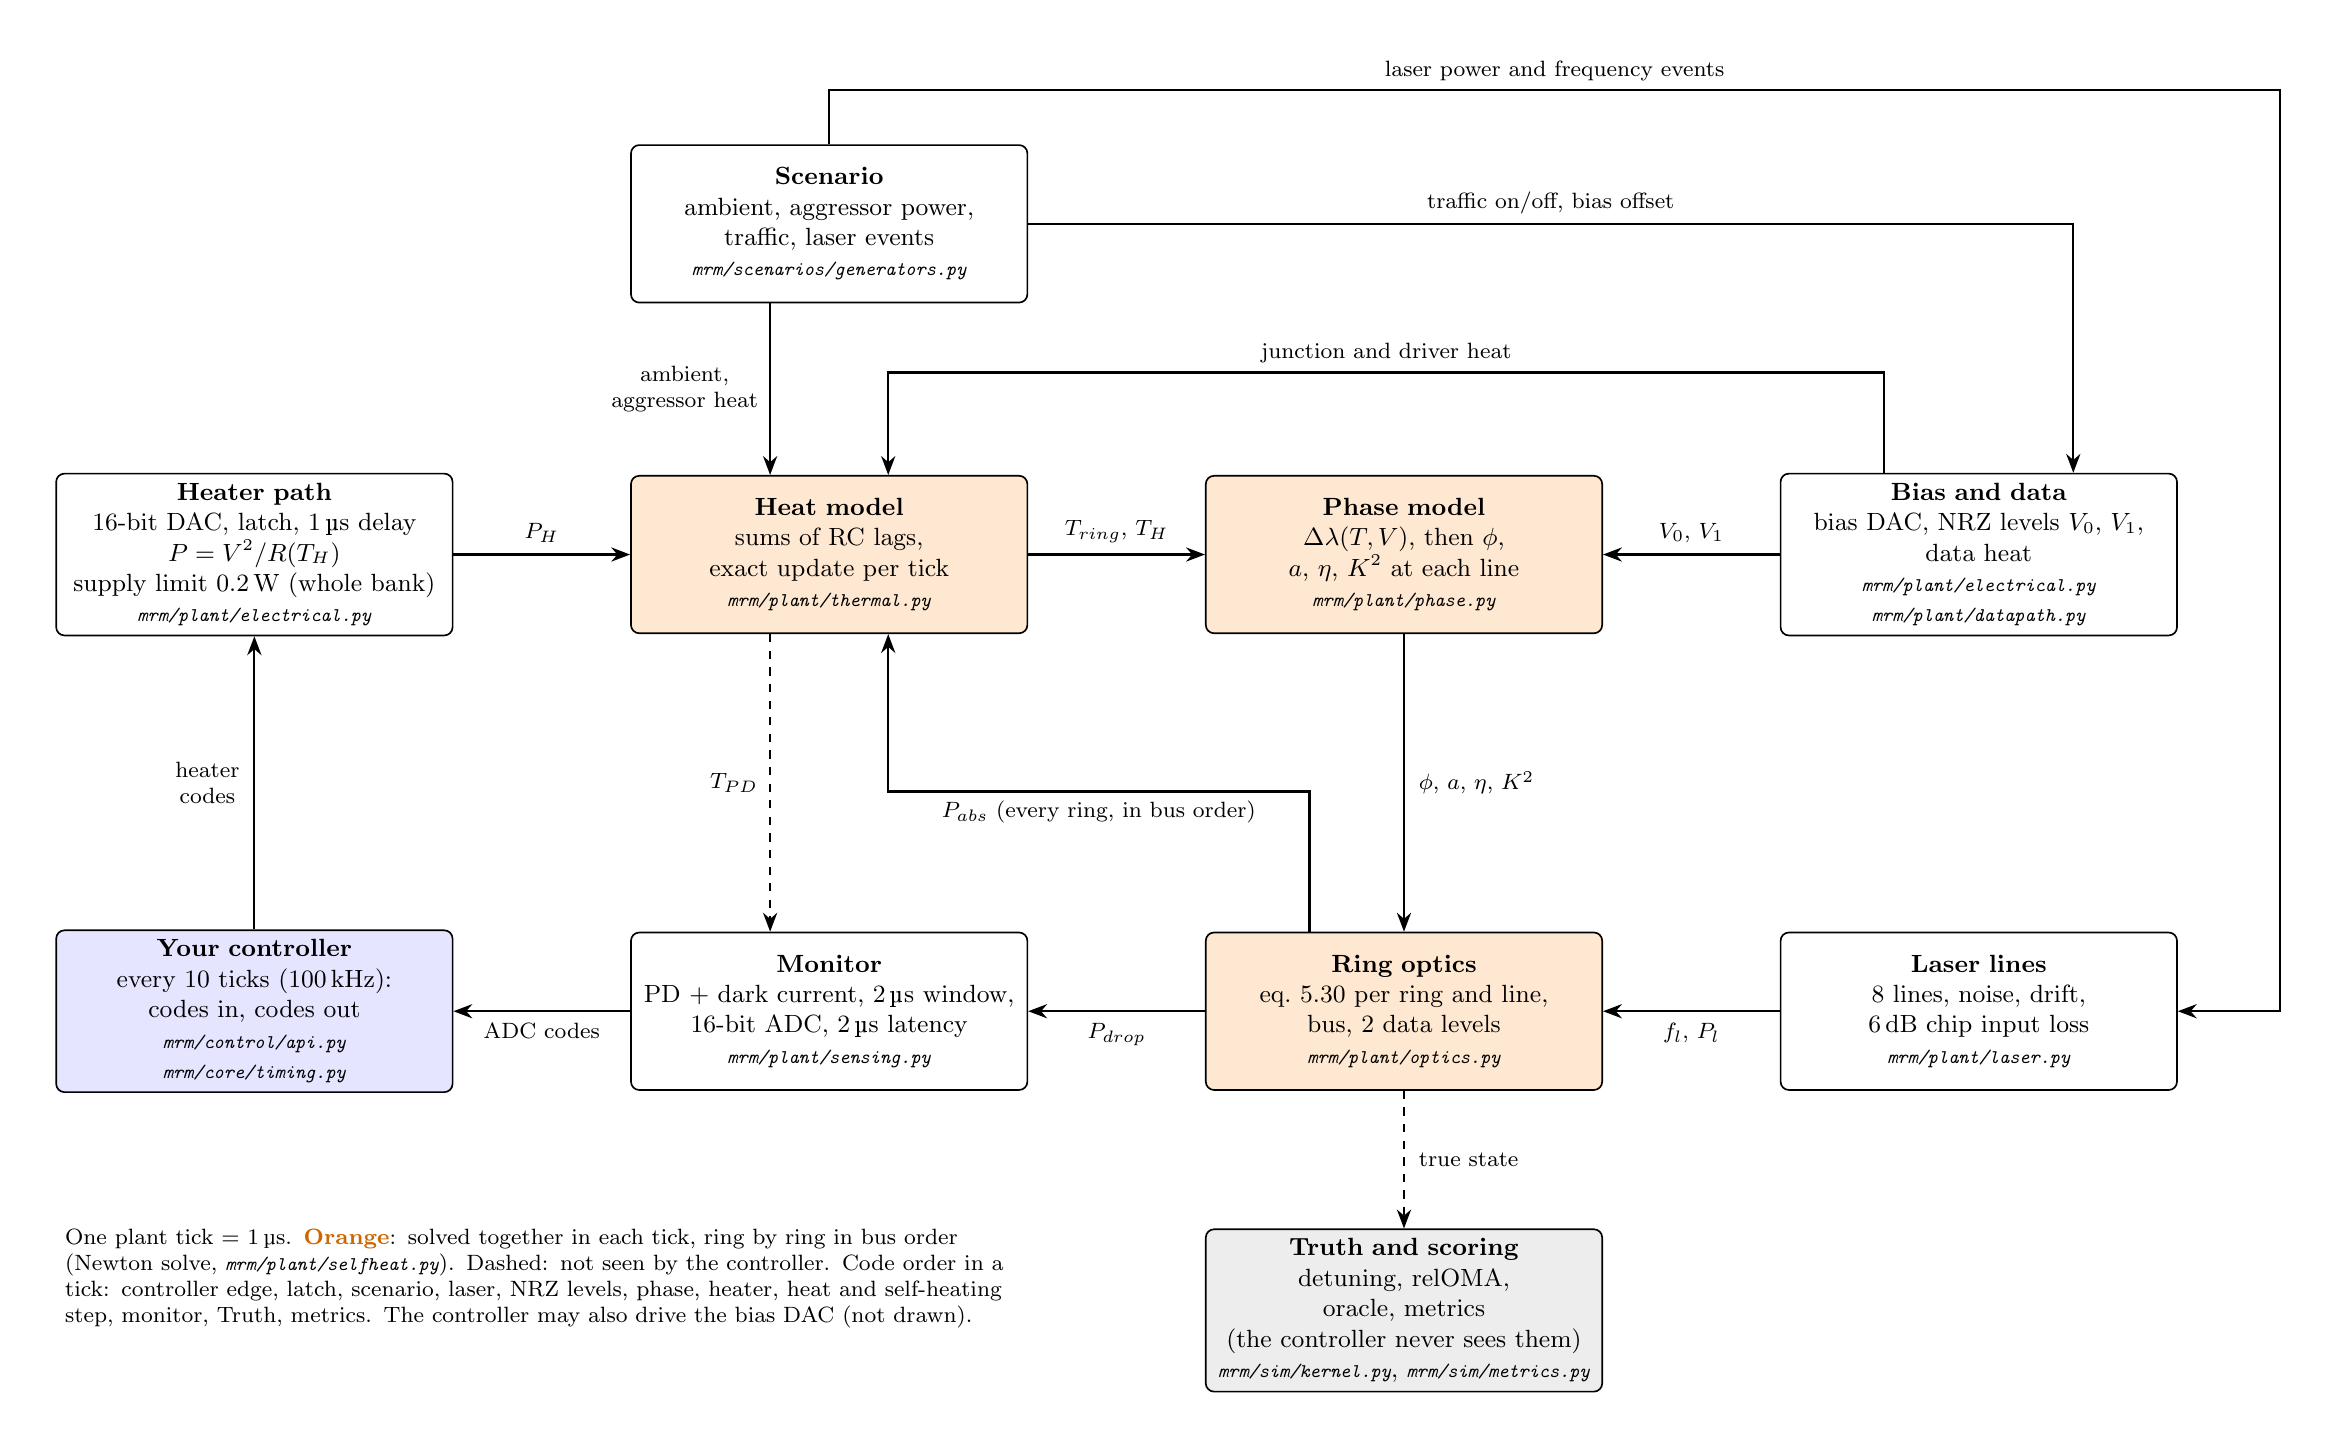
\begin{tikzpicture}[
    show background rectangle,
    background rectangle/.style={fill=white},
    inner frame sep=10pt,
    blk/.style={draw, rounded corners=3pt, align=center, font=\small, text width=4.8cm, minimum height=2.0cm,
                fill=#1, line width=0.6pt},
    blk/.default=white,
    arr/.style={-{Stealth[length=2.4mm]}, line width=0.8pt},
    hid/.style={arr, dashed},
    lab/.style={font=\footnotesize, inner sep=2pt, align=center, fill=white},
  ]
  % ---------------------------------------------------------------------------------------------- the control loop
  \node[blk]           (heat)  at (0,0)    {\textbf{Heater path}\\16-bit DAC, latch, 1\us{} delay\\
                                            \mbox{$P=V^2/R(T_H)$}\\supply limit 0.2\,W (whole bank)\\
                                            \file{mrm/plant/electrical.py}};
  \node[blk=orange!18] (therm) at (7.3,0)  {\textbf{Heat model}\\sums of RC lags,\\exact update per tick\\
                                            \file{mrm/plant/thermal.py}};
  \node[blk=orange!18] (ph)    at (14.6,0) {\textbf{Phase model}\\$\Delta\lambda(T,V)$, then $\phi$,\\
                                            $a$, $\eta$, $K^2$ at each line\\\file{mrm/plant/phase.py}};
  \node[blk=orange!18] (opt)   at (14.6,-5.8) {\textbf{Ring optics}\\eq.~5.30 per ring and line,\\
                                            bus, 2 data levels\\\file{mrm/plant/optics.py}};
  \node[blk]           (mon)   at (7.3,-5.8) {\textbf{Monitor}\\PD + dark current, 2\us{} window,\\
                                            16-bit ADC, 2\us{} latency\\\file{mrm/plant/sensing.py}};
  \node[blk=blue!10]   (ctrl)  at (0,-5.8) {\textbf{Your controller}\\every 10 ticks (100\,kHz):\\
                                            codes in, codes out\\\file{mrm/control/api.py}\\\file{mrm/core/timing.py}};

  \draw[arr] (heat) -- node[lab, above=2pt]{$P_H$} (therm);
  \draw[arr] (therm) -- node[lab, above=2pt]{$T_{ring}$, $T_H$} (ph);
  \draw[arr] (ph) -- node[lab, right=3pt, fill=none]{$\phi$, $a$, $\eta$, $K^2$} (opt);
  \draw[arr] (opt) -- node[lab, below=2pt]{$P_{drop}$} (mon);
  \draw[arr] (mon) -- node[lab, below=2pt]{ADC codes} (ctrl);
  \draw[arr] (ctrl) -- node[lab, left=3pt, fill=none]{heater\\codes} (heat);

  % inside the loop: optical self-heating and the PD temperature
  \draw[arr] ($(opt.north)+(-1.2,0)$) |- ($(therm.south)+(0.75,-2.0)$)
        node[lab, pos=0.75, below=1pt, fill=none]{$P_{abs}$ (every ring, in bus order)} -- ($(therm.south)+(0.75,0)$);
  \draw[hid] ($(therm.south)+(-0.75,0)$) -- node[lab, left=2pt, fill=none]{$T_{PD}$} ($(mon.north)+(-0.75,0)$);

  % ------------------------------------------------------------------------------------------- inputs from outside
  \node[blk]           (scen)  at (7.3,4.2)  {\textbf{Scenario}\\ambient, aggressor power,\\traffic, laser events\\
                                              \file{mrm/scenarios/generators.py}};
  \node[blk]           (bias)  at (21.9,0)   {\textbf{Bias and data}\\bias DAC, NRZ levels $V_0$, $V_1$,\\data heat\\
                                              \file{mrm/plant/electrical.py}\\\file{mrm/plant/datapath.py}};
  \node[blk]           (las)   at (21.9,-5.8) {\textbf{Laser lines}\\8 lines, noise, drift,\\6\,dB chip input loss\\
                                              \file{mrm/plant/laser.py}};

  \draw[arr] ($(scen.south)+(-0.75,0)$) -- node[lab, left=2pt, fill=none]{ambient,\\aggressor heat}
        ($(therm.north)+(-0.75,0)$);
  \draw[arr] (bias) -- node[lab, above=2pt]{$V_0$, $V_1$} (ph);
  \draw[arr] ($(bias.north)+(-1.2,0)$) |- ($(therm.north)+(0.75,1.3)$)
        node[lab, pos=0.75, above=1pt, fill=none]{junction and driver heat} -- ($(therm.north)+(0.75,0)$);
  \draw[arr] (scen.east) -| node[lab, pos=0.25, above=1pt, fill=none]{traffic on/off, bias offset}
        ($(bias.north)+(1.2,0)$);
  \draw[arr] (scen.north) |- ($(las.east)+(1.3,11.7)$) node[lab, pos=0.75, above=1pt, fill=none]{laser power and
        frequency events} |- (las.east);
  \draw[arr] (las) -- node[lab, below=2pt]{$f_l$, $P_l$} (opt);

  % ------------------------------------------------------------------------------- what the controller never sees
  \node[blk=gray!14]   (truth) at (14.6,-9.6) {\textbf{Truth and scoring}\\detuning, relOMA, oracle, metrics\\
                                              (the controller never sees them)\\
                                              \file{mrm/sim/kernel.py}, \file{mrm/sim/metrics.py}};
  \draw[hid] (opt) -- node[lab, right=3pt, fill=none]{true state} (truth);

  % ------------------------------------------------------------------------------------------------------ legend
  \node[font=\footnotesize, align=left, anchor=north west, text width=12cm] at ($(ctrl.south west)+(0,-1.6)$)
    {One plant tick = 1\us. \textcolor{orange!80!black}{\textbf{Orange}}: solved together in each tick, ring by
     ring in bus order (Newton solve, \file{mrm/plant/selfheat.py}). Dashed: not seen by the controller.
     Code order in a tick: controller edge, latch, scenario, laser, NRZ levels, phase, heater, heat and
     self-heating step, monitor, Truth, metrics. The controller may also drive the bias DAC (not drawn).};
\end{tikzpicture}
\end{document}
